%%
%% This is file `mcmthesis-demo.tex',
%% generated with the docstrip utility.
%%
%% The original source files were:
%%
%% mcmthesis.dtx  (with options: `demo')
%% 
%% -----------------------------------
%% 
%% This is a generated file.
%% 
%% Copyright (C)
%%       2010 -- 2015 by Zhaoli Wang
%%       2014 -- 2019 by Liam Huang
%%       2019 -- present by latexstudio.net
%% 
%% This work may be distributed and/or modified under the
%% conditions of the LaTeX Project Public License, either version 1.3
%% of this license or (at your option) any later version.
%% The latest version of this license is in
%%   http://www.latex-project.org/lppl.txt
%% and version 1.3 or later is part of all distributions of LaTeX
%% version 2005/12/01 or later.
%% 
%% This work has the LPPL maintenance status `maintained'.
%% 
%% The Current Maintainer of this work is latexstudio.net.
%% 
%%
%% This is file `mcmthesis-demo.tex',
%% generated with the docstrip utility.
%%
%% The original source files were:
%%
%% mcmthesis.dtx  (with options: `demo')
%%
%% -----------------------------------
%%
%% This is a generated file.
%%
%% Copyright (C)
%%       2010 -- 2015 by Zhaoli Wang
%%       2014 -- 2019 by Liam Huang
%%       2019 -- present by latexstudio.net
%%
%% This work may be distributed and/or modified under the
%% conditions of the LaTeX Project Public License, either version 1.3
%% of this license or (at your option) any later version.
%% The latest version of this license is in
%%   http://www.latex-project.org/lppl.txt
%% and version 1.3 or later is part of all distributions of LaTeX
%% version 2005/12/01 or later.
%%
%% This work has the LPPL maintenance status `maintained'.
%%
%% The Current Maintainer of this work is Liam Huang.
%%
\documentclass{mcmthesis}
\mcmsetup{CTeX = false,   % 使用 CTeX 套装时,设置为 true
        tcn = 2101675, problem = A,
        sheet = true, titleinsheet = true, keywordsinsheet = true,
        titlepage = false, abstract = true}
\usepackage{newtxtext}%\usepackage{palatino}
\usepackage{lipsum}

\title{The Modeling and Simulation of Fungi Decomposition Process}
\author{\small \href{2101675}
  {\includegraphics[width=7cm]{mcmthesis-logo}}}
\date{\today}
\graphicspath{{img/}}
\usepackage{graphicx}
\usepackage{subfigure}
\usepackage{float}
\usepackage{color}
\definecolor{codegreen}{rgb}{0,0.6,0}
\definecolor{codegray}{rgb}{0.5,0.5,0.5}
\definecolor{codepurple}{rgb}{0.58,0,0.82}
\definecolor{backcolour}{rgb}{0.95,0.95,0.92}
\usepackage{indentfirst}
\usepackage{tocloft} 
%\renewcommand{\cftchapleader}{\cftdotfill{\cftdotsep}}
\renewcommand{\cftsecleader}{\cftdotfill{\cftdotsep}}
\lstset{
	backgroundcolor=\color{backcolour},   
	commentstyle=\color{codegreen},
	keywordstyle=\color{magenta},
	numberstyle=\tiny\color{codegray},
	stringstyle=\color{codepurple},
	basicstyle=\footnotesize,
	breakatwhitespace=false,         
	breaklines=true,                 
	captionpos=b,                    
	keepspaces=true,                 
	numbers=left,                    
	numbersep=5pt,                  
	showspaces=false,                
	showstringspaces=false,
	showtabs=false, 
	%escapebegin=\begin{CJK*}{GBK}{hei},escapeend=\end{CJK*},                 
	tabsize=2
}
\usepackage{lastpage}
\begin{document}
\begin{abstract}

Fungi decomposition of litter is often a very complex process, which involves many external and internal factors. If many factors are considered, the established model will be very complex. To this end, our goal is to reduce the influencing factors, establish a simplified model of litter decomposition in a given area. 

First of all, according to the description of reference, we know that there is a certain correlation between the decomposition rate and the growth rate and moisture tolerance of fungi. We use decomposition rate as dependent variable, growth rate and moisture tolerance as independent variables to establish a functional relationship between the three. On the basis of this relationship, we establish litter decomposition model with litter residue as dependent variable, decomposition rate and time as independent variables. There are three types of litter decomposition model : positive exponential decline model, Logistic model, and improved Olson negative exponential decline model.

Then, the Lotka-Volterra competition model between strains was established. We mapped the variables such as fungal population growth rate, environmental capacity, fungal growth rate, moisture tolerance, and temperature. The total number of individuals in the population was used to reflect the decomposition rate, and an improved Lotka-Volterra competition model was established to describe the relationship between ( population growth and decomposition ) and ( growth rate, moisture tolerance, and time ). 

In addition, in order to study the relationship between the number of litters and the growth rate and moisture tolerance of fungi in the presence of competition, we adopted the strategy of fixing one independent variable and studying the relationship between the other independent variable and the dependent variable. The ratio of the growth rate of the two fungi was set to have different sizes. The moisture tolerance was treated by the same method. The relevant parameter values were substituted into the equations for simulation experiments to obtain the population growth and decomposition under different ratios, and then the comparative analysis was carried out.

Based on the above experimental results, we analyzed the overall trend, short-term and long-term trends, and found that there were positive and negative competition between the two fungal populations under different parameters, which promoted and hindered the decomposition of litter, respectively. Based on the experimental results, we also analyzed the sensitivity of rapid environmental fluctuations, predicted the species with relative advantages and disadvantages, predicted the decomposition under various environmental conditions ,discussed the impact of biodiversity on decomposition, and analyzed the sensitivity of the model.

%Finally, we discussed the impact of biodiversity on decomposition, analyzed the sensitivity of the model, and described the strengths and weaknesses of the model and the improvement direction.

\begin{keywords}
Differential Equation ; Olson Model ;Lotka-Volterra Model ;Interspecific Competition
\end{keywords}
\end{abstract}
\maketitle
%% Generate the Table of Contents, if it's needed.
%% \tableofcontents
%% \newpage
%%
%% Generate the Memorandum, if it's needed.
%% \memoto{\LaTeX{}studio}
%% \memofrom{Liam Huang}
%% \memosubject{Happy \TeX{}ing!}
%% \memodate{\today}
%% \logo{\LARGE I'm pretending to be a LOGO!}
%% \begin{memo}[Memorandum]
%%   \lipsum[1-3]
%% \end{memo}
%%

\newpage
\tableofcontents
\thispagestyle{empty}


\newpage
\setcounter{page}{1}
\section{Introduction}
\subsection{Background}
The carbon cycle describes the process of carbon exchange throughout the Earth's geochemical cycle and is an important part of life on Earth. A part of the carbon cycle includes the decomposition of compounds, which enables carbon to be updated and used in other forms. A key component of this process is the decomposition of plant materials and lignocellulose. 

Some of the key factors in decomposing lignocellulose are fungi. The authors of a recent research paper on fungal decomposition of wood identified fungal characteristics that determine the decomposition rate, and pointed out the links between some characteristics . In particular, fungal strains with slow growth can survive and grow better under the condition of environmental changes such as humidity and temperature, while strains with faster growth often cannot grow robustly under the same changes.

These researchers studied a large number of traits related to different fungi and their roles in the decomposition of ground litter ( dead plant materials ) and lignocellulose.
\subsection{Restatement of problem}

Our main goal is to establish a model for the decomposition of lignocellulose on a given land, and to model in the case of the existence of multiple fungal decomposition types of lignocellulose in the same region. 

When exploring the relationship between these two interesting properties, namely growth rate and moisture tolerance, and decomposition rate, several questions may arise : 

How do different fungi interact in different environments and decompose ground litter in fixed plots using these two properties ? In these different environments, how will decomposition be affected with the change of conditions ? How do environmental changes in specific environments and how do environmental changes affect long-term dynamics of fungal decomposition and competition ? 

Therefore, we need to explore and solve the following aspects. 

A mathematical model need to be established to describe the decomposition of ground litter and lignocellulose through fungal activities in the presence of various fungi. 

In your model, the interactions between different types of fungi need to be included. These fungi have different growth rates and different moisture tolerances. 

Provide model analysis and describe the interaction between different types of fungi. The dynamic characteristics and description of interaction should include short-term and long-term trends. Your analysis should examine sensitivity to rapid environmental fluctuations and determine the overall impact of changes in atmospheric trends to assess the impact of changes in local weather patterns.
It includes the prediction of the relative advantages and disadvantages of each species and possible persistent species combination, as well as the prediction of different environments such as drought, semi-arid, temperate, arboreal and tropical rainforest.

Describes how the diversity of fungal communities in a system affects the overall efficiency of the system in litter decomposition. When there are varying degrees of variation in the local environment, the importance and role of biodiversity prediction. 

Two pages of article are needed to be attached to the results. In discussing the latest progress in our understanding of the role of fungi in ecosystems, your article should be suitable as an introductory textbook for college biology.
\subsection{Our Work}
\begin{itemize}
\item Establishment of positive exponential decline model between litter residue and time, Logistic model and improved Olson negative exponential decline model.

\item The Lotka-Volterra competition model between strains was established to reflect the decomposition rate by the total number of individuals.

\item The growth rate and moisture tolerance parameters were substituted for simulation experiments to obtain the population growth and decomposition under different ratios for comparative analysis.

\item Analyze the overall trend, short-term and long-term trends, analyze the sensitivity of rapid environmental fluctuations, predict the relative advantages and disadvantages of species, and predict the decomposition of different environmental conditions.
\end{itemize}
\section{General Assumptions and Symbol Description}
\subsection{General Assumptions}
The process of fungal decomposition of litter is often very complex. We simplify the model as much as possible and assume that some parameters are used for theoretical analysis rather than data fitting. In our model, the dependent variable is the residual biomass, the independent variable is time and decomposition rate, and the decomposition rate is related to other environmental external factors and fungal factors. When discussing multi-species interactions, we only deal with the competitive relationship between two species with different characteristics. In order to better establish our model, we make the following assumptions :
\begin{itemize}
\item Decomposition rate is proportional to fungal growth rate and temperature.

\item The logarithm of decomposition rate is inversely proportional to the moisture tolerance of fungi.

\item Resources in the environment are limited.
\end{itemize}
\subsection{Symbol Description}
\begin{table}[H]
	\centering
	\begin{tabular}{cc}
		\toprule[1.5pt]
		Symbol & Description \\
		\midrule
		$D$ & Decomposition rate \\
		$M$ & Moisture tolerance of fungi\\
		$R$ & Fungal growth rate\\
		$S$ & The residual amount of ground litter \\
		$S_m$ &  The initial amount of ground litter\\
		$t$ &  Time\\
		$x,y$ &  Amount of two species\\
		$n_1,n_2$ &  Environmental capacity of two species\\
		$k$ &  Ratio of growth rates of two species\\
		$h$ &  Ratio of moisture tolerance of two species\\
		$Sum$ &  Total population growth rate of two species\\
		$Q$ &  Total amount of individuals of two species\\
		$\alpha,\beta,\eta$ &  Relevant proportional coefficient\\
		
		\bottomrule[1.5pt]
	\end{tabular}%
\end{table}%
\section{Establishment of Single Species Model}
Considering that the dependent variable is the residual amount of ground litter, and the independent variables are time, moisture tolerance and growth rate, the corresponding relationship can be investigated first.

We first consider the intermediate variable decomposition rate D, t is time, R is growth rate, M is moisture tolerance. It is necessary to solve the functional expression for each type of fungi. The decomposition rate D is related to the growth rate and moisture tolerance. In the single species model, we assume that the decomposition rate is independent of time, but is a constant related to the growth rate and moisture tolerance. Therefore, the following functional relationship is constructed :
$$D=F(M,R)$$
F(M,R) is the function of M, R. It represents the combined effect of M, R on decomposition rate, and its value is exactly equal to the relative decomposition rate of litter decomposition.
It can be seen from the figure that the logarithm of decomposition rate is negatively correlated with the moisture tolerance index, and the decomposition rate is positively correlated with the growth rate. After analysis and calculation, F ( M, R ) takes a linear form. From the experimental data, it can well describe the dynamic law of litter decomposition, and has a simple form :
$$F(M,R)=a-b e^{kM}+c R$$
\\
\\
The relationship between decomposition rate D and the amount of ground litter is discussed below :

\textbf{1.} \quad Cui-Lawson single population model based on nutritional dynamics usually takes the form of :
$$	\frac{d x}{x d t}=\mu_{c} \frac{1-x / x_{m}}{1-x / x_{m}^{\prime}}$$

In the formula,x is microbial population density, $x_{m}^{\prime}$is maximum population density that microbial populations may reach after all ground litter are utilized by microorganisms,$ x_{a}^{\prime}-x_{m}+k / \alpha, \mu_{c}=\frac{x_{m}}{x_{m}^{\prime}} \mu_{m}$
,where,$ \mu_{m}$is intrinsic growth rate of microbial population growth,k is the Michalis-Menten constant,(Michalis-Menten constant),microbial population growth rate$\left(\frac{d x}{x dt}\right)$ reaches$1 / 2 \mu_{m}$the amount of ground litter,$\boldsymbol{\alpha}$is 'Equivalence' of converting ground litter into microbial cells,besides,$\mathcal{S}_{m}-S=\alpha x, S_{m}=\dot{\alpha} x_{m}$
where,$S_m$ is the initial amount of ground litter;S is the residual amount of ground litter,$S_m-S$is amount of Bioresidues Decomposed by Microorganisms。
If the variable x (microbial population density) in Formula (1) is replaced by S  (number of ground litter),$\mu_{m}$is replaced by$D=F(M,R)$,the Cui-Lawson model can be rewritten to:
$$	
\begin{array}{l}
	-\frac{d s}{s d t}=D \frac{S_{m}-S}{K+S} \vspace{2ex}  \\ 
	\frac{K+S}{\left(S_{m}-S\right) S} d s=D d t
\end{array}
$$
After separating variables,$$\frac{K}{S_{m}}\left[\frac{1}{S}+\frac{1}{S_{m}-S}\right] d s+\frac{d s}{S_{m}-S}=-D d t$$

After integration:$$\frac{K}{S_{m}} \ln \frac{S}{S_{0}}-\frac{K}{S_{m}} \ln \frac{S_{m}-S}{S_{m}-S_{0}}-\ln \frac{S_{m}-S}{S_{m}-S_{0}}=-D t$$

This is the biological decomposition model of organic residues based on nutritional kinetics.
When$K / S_{m} \rightarrow 0$, equation is

$$\frac{S_{m}-S}{S_{m}-S_{0}}-e^{D t}$$

$$S=S_{m}-\left(S_{m}-S_{0}\right) e^{D t}$$

The second term$\left({S}_{m}-S_{0}\right) e^{D t}$on the right side of the formula here obviously increases exponentially with time, indicating that the rate of reduction of ground litter, that is, the rate of decomposition and utilization of microorganisms increases exponentially. Therefore, the change of ground litter S presents a trend of complementarity with the exponential growth, which can be called the exponential complementarity type. The change curve of this model is shown in the solid line in Fig.1, and the dotted line in the figure is exactly the exponential curve of the growth of microbial population to absorb nutrients. The two curves are complementary, and the total is$S_m$



The condition of exponential complementarity is$K/S_m→0$, that is, the initial amount of ground litter $S_m$ is very large ( fully meeting the initial amount of microbial population $S_m$ is very large ), and fully meeting the requirements of exponential growth of microbial population, which is in many cases in line with the actual situation.

When$K / S_{m} \rightarrow \infty$,equation is translated into :
$$S=\frac{S_{m}}{1+\frac{S_{m}-S_{0}}{S_{0}} \exp \left[\frac{S_{m}}{K} D t\right]}$$

At this time, the growth of microbial population ( absorbing nutrients ) showed a Logistic curve, so the decomposition model of ground litter was complementary to the Logistic curve. 
\begin{figure}[H]
	\centering
	\subfigure[Model curve A of bio-residue decomposition based on nutrition dynamics and exponential growth curve of microbial population]{
		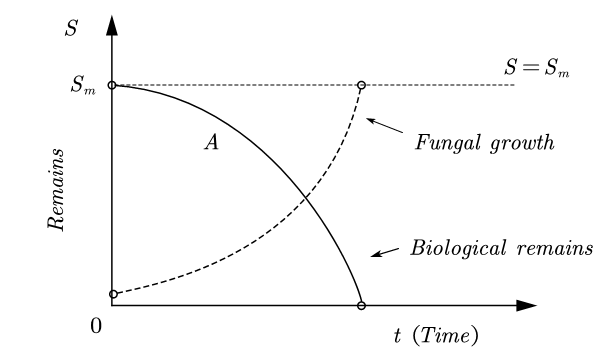
\includegraphics[width=0.6\linewidth]{img/指数增长模型.png}
		%\caption{fig1}
	}
	\quad
	\subfigure[Bioresidue decomposition model curve based on nutritional dynamics  B and Logistic Growth Curve of Microbial Population]{
		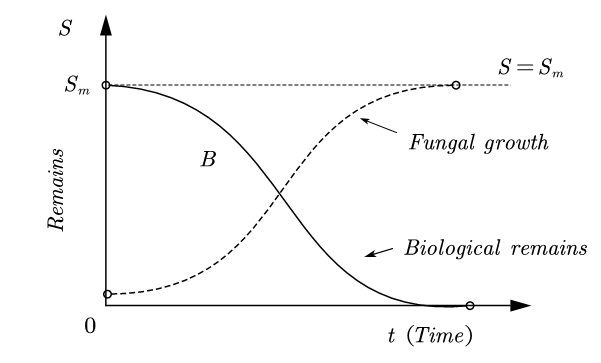
\includegraphics[width=0.6\linewidth]{img/logistic模型.png}
	}
	\caption{The decomposition model curves of kinds of ground litter and the growth curves of microbial population}
	\label{fig:jiago}
\end{figure} 

With the change of $K/S_m$, equation can be expressed by a set of curves, which are between curves A and B. In addition, when $K/S_m=1$, curve C is shown in Fig. 2, which can be called the complementary type of Cui-Lawson growth curve.
\begin{figure}[H]
	\centering
	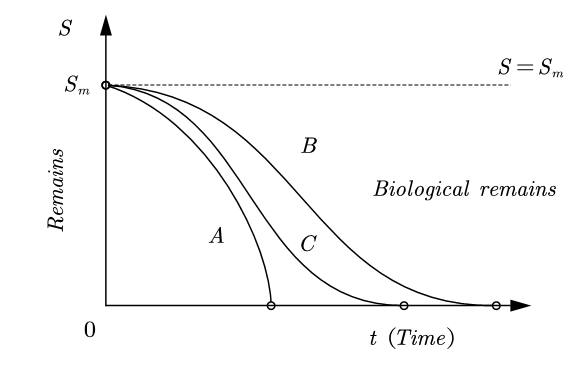
\includegraphics[width=0.6\textwidth]{img/3种不同的曲线.png}
	\caption{Different forms of decomposition models A, B, C of ground litter}\label{fig:3种不同的曲线}
\end{figure}
\textbf{2.} \quad Another model of biomass residue quantity and decomposition rate is the improved Olson single exponential decay model. t Represents time and $S$ represents residues of the litter at time t (g)

$-\frac{\mathrm{d} S}{\mathrm{d} t}$is the absolute decomposition rate of litter. measured by the weight of litter decomposition per unit time.; $-\frac{\mathrm{d} S}{\mathrm{d} t} / S$is the relative decomposition rate of litter, measured by the weight of litter decomposition per unit weight in unit time. It is assumed that the absolute decomposition rate of litter is proportional to the residual amount and is proportional to the function $ D = F ( M, R ) $ of moisture tolerance M and mycelium growth rate R, because the greater the residual amount of litter, the greater the total weight of decomposition per unit time. So
$$\frac{d S}{d t}=-D S$$
F( M, R ) is the function of M, R. It represents the combined effect of M, R on decomposition rate, and its value is exactly equal to the relative decomposition rate of litter decomposition.

So we can get:$$\frac{S}{S_m}=e^{-D t}$$
Where:$$D=F(M,R)$$
Assuming that the decomposition rate D is a constant, the relationship between the number of ground litter and time is as follows ;
\begin{figure}[H]
	\centering
	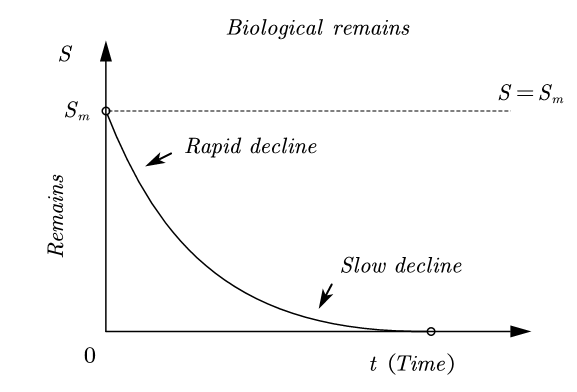
\includegraphics[width=0.7\textwidth]{img/olson模型.png}
	\caption{Improved Olson Model}\label{fig:olson模型}
\end{figure}
\section{Establishment of Multi-Species Model}
The interactions among strains include competition, symbiosis, parasitism, predation, and parasitism, but the competition should be focused on.             

When the two populations compete for the same food source and living space, the common outcome is the extinction of weak competitiveness, and strong competitiveness reaches the maximum capacity allowed by the environment. The population competition model can be used to describe the process of competition between two populations and analyze the conditions of various outcomes.

\subsection{Lotka-Volterra Model}
The competitive relationship between two populations living in the same natural environment is studied. It is assumed that the number evolution of the two populations living alone in this natural environment follows the Logistic law, and that when they compete with each other, the growth of each other will be slowed down, and the decrease of growth rate is proportional to the product of their number. The ordinary differential equation model established according to this assumption is 

 $$\frac{d x}{d t}=r_{1} x\left(1-\frac{x}{n_{1}}\right) \quad \frac{d y}{d t}=r_{1} y\left(1-\frac{y}{n_{1}}\right)$$
 
x, y : Populations of two species

n1, n2 : Environmental capacity of two species             

r1, r2 : Population growth rates for two species             

When the two groups survive together, the blocking effect of B on the growth of A is proportional to the number of B ; A has the same effect on B.
$$\frac{d x}{d t}=r_{1} x\left(1-\frac{x}{n_{1}}-s_{1} \frac{y}{n_{2}}\right)$$ 
$$\frac{d y}{d t}=r_{2} y\left(1-\frac{y}{n_{2}}-s_{2} \frac{x}{n_{1}}\right)$$
The meaning of s1 is that the consumption of unit number of B ( relative n2 ) is s1 times that of unit number of A ( relative n1 ) for the resources of supply A, s2 is the same. Under the effect of competition, the population growth is no longer a simple exponential curve or Logistic curve, and may change the proportion and growth rate of various populations with the change of competition factors and environment.
\subsection{Improved Lotka-Volterra model}
We noticed that the slow-growing fungal strains can often survive and grow better under environmental changes such as humidity and temperature, while the fast-growing strains cannot grow robustly against the same changes, indicating that the competitive factor s of the two different fungal populations is related to the growth rate, and the relationship between them is $s=g(R)$ ,Environmental capacity is also related to moisture tolerance, and its functional relationship is set as $ n = h ( M ) $. Population growth rate r is described by fungal growth rate R itself. For simplicity, we set the relationship between $ g ( R ) $, $ h ( M ) $ as linear, that is, $$s=\alpha R,n=\beta M$$

Then the equation set of the model becomes :

$$\frac{d x}{d t}=R_{1} x\left(1-\frac{x}{\beta M_{1}}-\alpha R_{1} \frac{y}{\beta M_{2}}\right)$$ 
$$\frac{d y}{d t}=R_{2} y\left(1-\frac{y}{\beta M_{2}}-\alpha R_{2} \frac{x}{\beta M_{1}}\right)$$

This is the relationship equation between the number of two populations and their growth rate and moisture tolerance.
\\
\\
Now we consider the relationship between the number of ground litter and time, strain growth rate, and moisture tolerance. We have a preliminary model for the first question.
$$\frac{d S}{d t}=-D S$$
We have previously assumed that the decomposition rate D has nothing to do with time t. However, in the competition model, the decomposition rate D becomes time dependent due to the interaction of multiple species, and the decomposition rate is proportional to the growth rate of the strain. We analogize the growth rate of the strain to the total population growth rate of the fungal community Sum.
$$D=F(M,R,t)=\eta * Sum(M,R,t)$$

So the equation$\frac{S}{S_m}=e^{-D t}$changes into$$\frac{S}{S_{m}}=e^{-\int D(t) d t}=e^{-\int F(M,R,t) d t}=e^{-\int \eta * Sum(M,R,t) d t}$$

$\eta$ is proportional coefficient,$$\int \eta * Sum(M,R,t) d t$$is the integral of the total population growth rate of fungal community, which is equivalent to the quantitative change of fungal community. Assuming that the total population is Q, the quantitative change function is$$Q(M,R,t)=x+y=x(M,R,t)+y(M,R,t)$$

So$$\frac{S}{S_m}=e^{-Q(M,R,t)}$$

Finally our integration model is
$$\left\{
\begin{array}{l}
	\frac{d x}{d t}=R_{1} x\left(1-\frac{x}{\beta M_{1}}-\alpha R_{1} \frac{y}{\beta M_{2}}\right)\\
	\frac{d y}{d t}=R_{2} y\left(1-\frac{y}{\beta M_{2}}-\alpha R_{2} \frac{x}{\beta M_{1}}\right)\\
	\frac{S}{S_m}=e^{-Q(M,R,t)}\\
	Q(M,R,t)=x+y=x(M,R,t)+y(M,R,t)\\
\end{array}
\right.
$$
\section{Analysis of Multi-Species Model}
In order to study the relationship between the number of ground litter and the growth rate and moisture tolerance of fungi in the presence of competition, we adopted the strategy of fixing one independent variable to study the relationship between another independent variable and the dependent variable.   When studying the relationship between any pair of variables, we make the following assumptions : the initial number of fungi in the population is the same. In order to facilitate the analysis, the following two kinds of simulation experiments set the second fungal growth rate and moisture tolerance higher.
\subsection{Relationship between the number of ground litter and growth rate}
Assuming that the two fungi have the same moisture tolerance, namely, $ M _ 1 = M _ 2 = M $, the environmental capacity of the two is equal. The growth rates of the two fungi can be measured by their proportional relationship, namely, $ R _ 2 = k * R _ 1 $. Then we set the relevant parameters and put them into the model to calculate the growth curve, the phase trajectory and the total population growth curve of the two fungi.       

When k is small ( k = 2 ), that is, when the growth rate of the two fungi is not much different, the curve is as follows :
\begin{figure}[H]
	\centering
	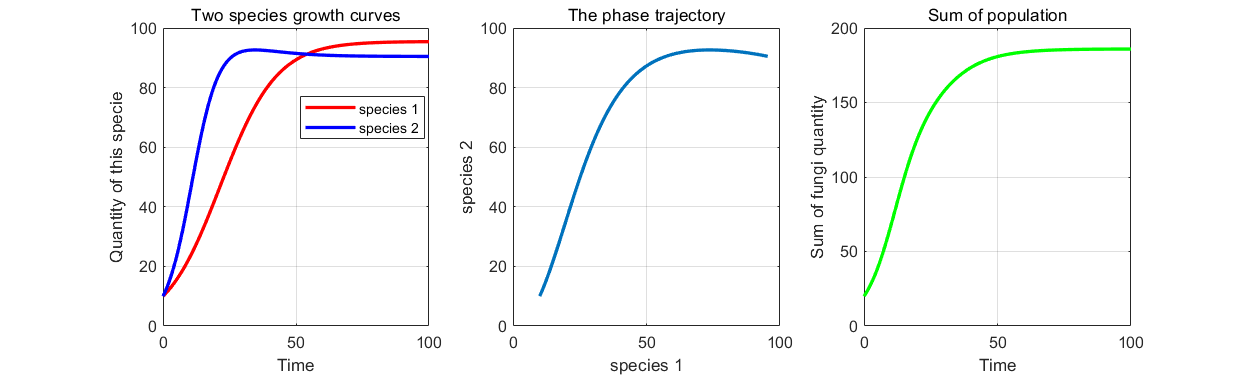
\includegraphics[width=1.0\textwidth]{img/k较小.png}
	\caption{3 Curves when k is small}\label{fig:k较小}
\end{figure}
When k is medium ( k = 10 ), that is, when the growth rate difference between the two fungi is in the intermediate state, the obtained curve is as follows :
 \begin{figure}[H]
	\centering
	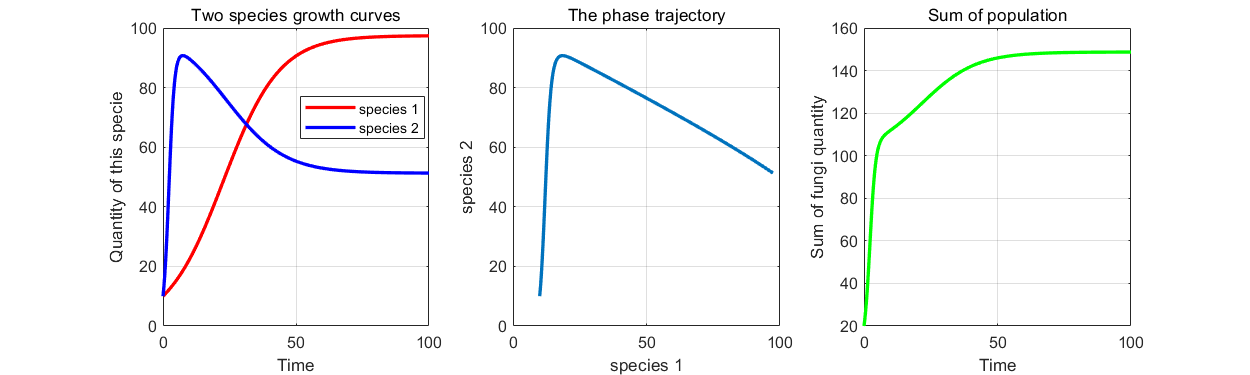
\includegraphics[width=1.0\textwidth]{img/k中等.png}
	\caption{3 Curves when k is medium}\label{fig:k中等}
\end{figure}
When k is big ( k = 50 ), that is, when the growth rate of the second fungi is far greater than that of the first one, the obtained curve is as follows :
\begin{figure}[H]
	\centering
	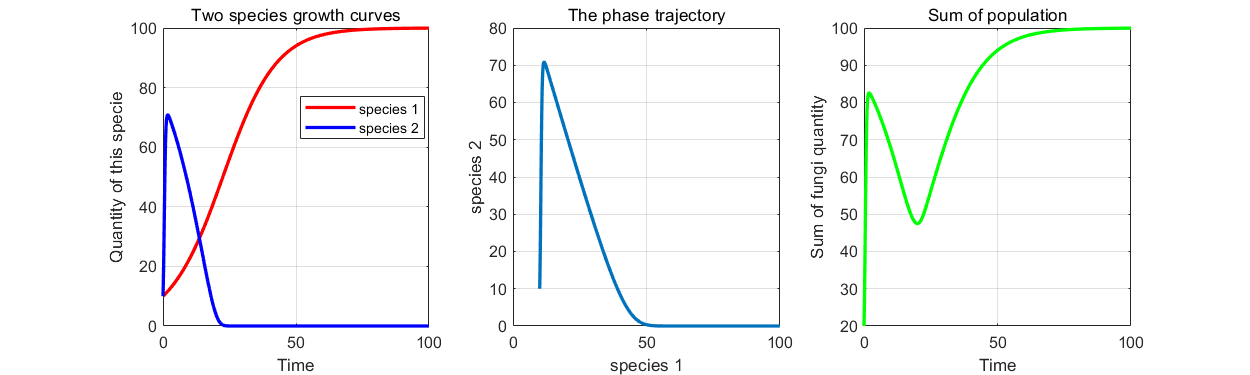
\includegraphics[width=1.0\textwidth]{img/k较大.png}
	\caption{3 Curves when k is big}\label{fig:k较大}
\end{figure}
Finally, the variation curves of the number of ground litter with time obtained under the above three conditions are as follows :
\begin{figure}[H]
	\centering
	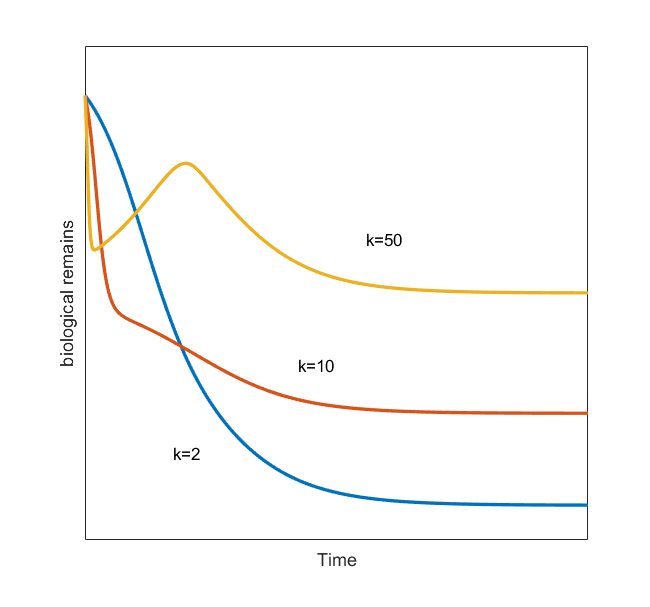
\includegraphics[width=0.6\textwidth]{img/不同k的分解曲线.png}
	\caption{Quantity Curves of ground litter under 3 k Values}\label{fig:不同k的分解曲线}
\end{figure}
\subsection{Relationship between the number of ground litter and moisture tolerance}
Similar to the first type of simulation experiments, assuming that the two fungi have the same growth rate, namely, $ R _ 1 = R _ 2 = R $, the growth rates of the two are equal. The relationship between the two moisture tolerances can be measured by their proportional relationship, namely $ M _ 2 = h * M _ 1 $. The environmental capacity n and the competition parameter s also have the corresponding proportional relationship. Then we set the relevant parameters and put them into the model to calculate the growth curve, the phase trajectory and the total population growth curve of the two fungi.       

When h is small ( h = 1.2 ), that is, when the moisture tolerance of the two fungi is not much different, the obtained curve is as follows :
\begin{figure}[H]
	\centering
	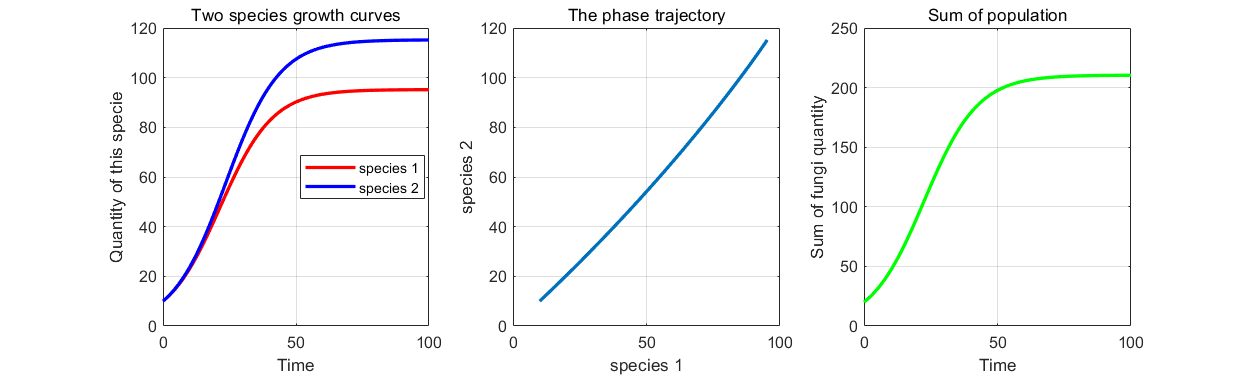
\includegraphics[width=1.0\textwidth]{img/h较小.png}
	\caption{3 Curves when h is small}\label{fig:h较小}
\end{figure}
When h is medium ( h = 10 ), that is, when the difference of moisture tolerance between the two fungi is in the intermediate state, the obtained curve is as follows :
\begin{figure}[H]
	\centering
	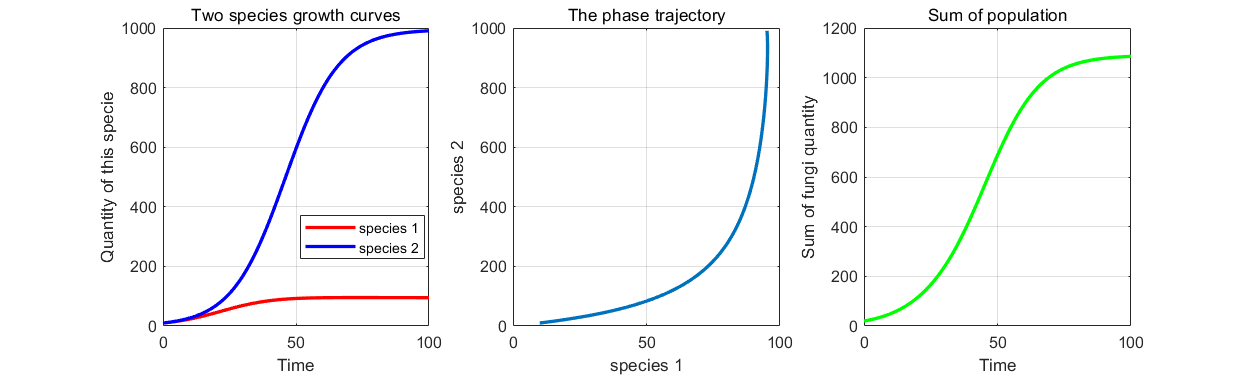
\includegraphics[width=1.0\textwidth]{img/h中等.png}
	\caption{3 Curves when h is medium}\label{fig:h中等}
\end{figure}
When h is big ( h = 50 ), that is, when the moisture tolerance of the second  fungi is much greater than that of the first, the curve is as follows :
\begin{figure}[H]
	\centering
	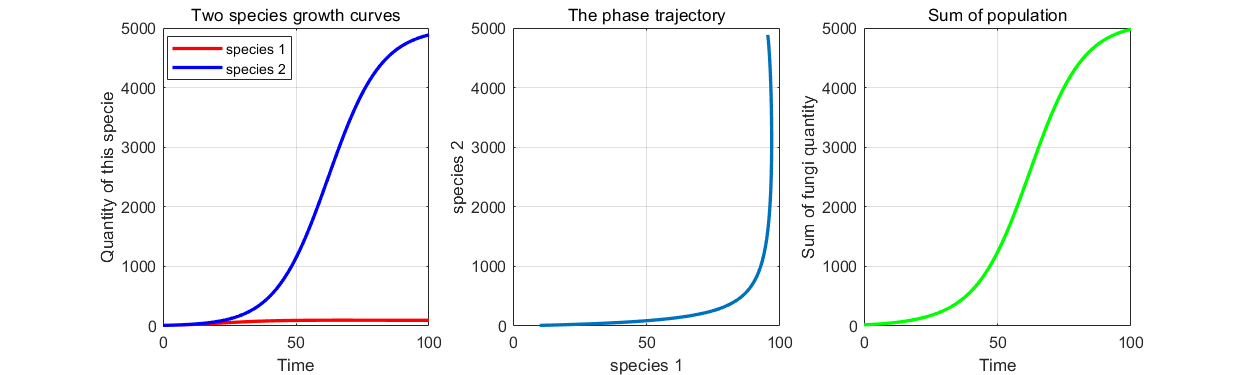
\includegraphics[width=1.0\textwidth]{img/h较大.png}
	\caption{3 Curves when h is big}\label{fig:h较大}
\end{figure}
Finally, the variation curves of the number of ground litter with time obtained under the above three conditions are as follows :
\begin{figure}[H]
	\centering
	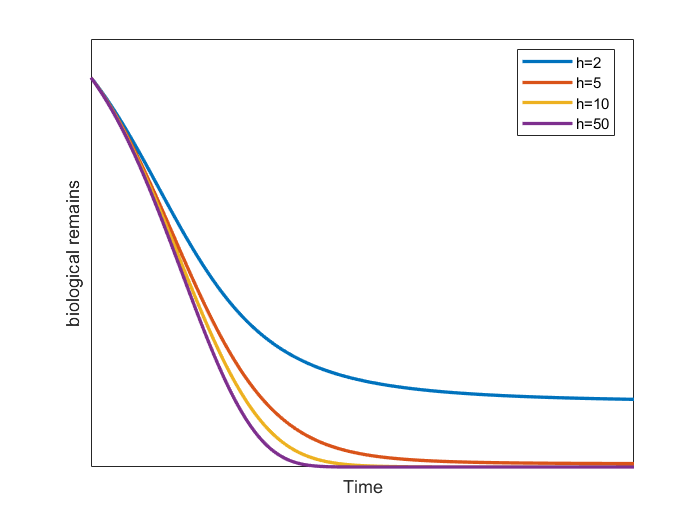
\includegraphics[width=0.6\textwidth]{img/不同h的分解曲线.png}
	\caption{Quantity Curves of ground litter under 4 h values}\label{fig:不同h的分解曲线}
\end{figure}
\subsection{Analysis of Model Result}
\subsubsection{Total Trend}
When the moisture tolerance was fixed, it can be seen that when k was small, the growth rates of the two fungi were not significantly different, and the final number level of the two species reached a consistent balance. The overall number of the two species increased steadily and the curve was smooth. When k is medium, the growth rate difference between the two fungi is in an intermediate state, and the final number levels of the two species are quite different, and the overall number growth of the two species has fluctuated. When k is large, i. e., the growth rates of the two fungi are quite different, it can be seen that the one with slower growth rate finally reaches the number balance, and the one with faster growth rate finally dies out. The overall number of the two increases first, then decreases and then increases, and finally reaches the balance.       

When the growth rate is fixed, unlike the first kind of simulation experiment, regardless of the size of h value, the number of the two fungi will eventually reach a variety of balance, and no longer extinction ;The overall number of both showed a steady S-shaped upward trend, only the final number size and the beginning of a rapid increase in time.
\subsubsection{Short-term and Long-term trends}
\textbf{1.} Fix moisture tolerance :       

No matter what kind of k value, the fungi with slow growth rate can always continue to grow. The fungi with fast growth rate grow rapidly in the short term, and the growth rate is much faster than that of the former. However, in the long run, as the process progresses, the number of fungi with fast growth will certainly decrease, and even lead to extinction when the growth rate varies greatly. For the overall growth of the two, when k is small and medium, the rapid growth in the short term, the final growth rate decreased, and finally reached constant ; When k is large, since the growth rate of fungi with fast growth rate is very large in the short term, and the number of fungi with slow growth rate begins to decline and extinction before rapid growth, the overall number of the two can grow rapidly in the short term, and then decline, and then begin to grow.      

For the decomposition of ground litter with different k values, the greater the k value is, the faster the decomposition is in the short term. However, in the long term, the faster the decomposition rate decreases, resulting in the greater the k value is, the less sufficient the decomposition is, which is a negative competition.

\textbf{2.} Fix growth rate :       

Under different moisture tolerance, the growth rate of the two fungi was slow at the beginning of a short period of time, and then the growth rate increased rapidly. In the long term, the growth rate of the two fungi decreased and the number reached stability.The overall number of the two also shows a slow-fast-slow trend. With the increase of h value, the time point for accelerating growth is delayed.       

For the decomposition of ground litter with different h values, the decomposition rate gradually increases in the short term, and then slows down. The final rate is 0, and the number of ground litter does not change. The greater the h, the greater the decomposition rate, the curve closer to the Y axis, and the more fully decomposed, which is a relatively positive competition.
\subsection{Sensitivity of rapid environmental fluctuations}
Comparison of sensitivity of temperature and humidity to decomposition rate :   We can know that temperature is related to the growth rate of fungi. Under the condition that fungi can grow, the higher the general temperature is, the greater the growth rate of fungi is. Fungal strains with slow growth can survive and grow better under the condition of environmental changes such as humidity and temperature, while strains with faster growth often cannot grow robustly under the same changes.      

When the ambient temperature is constant, the decomposition rate of fungi with obvious fast growth rate is faster ; When the ambient temperature changes rapidly, the fast-growing fungi grow rapidly in a short period of time, and then the number decreases in the competition because they do not adapt to the change of temperature, and the slow-growing fungi grow better. It can be known from our model that the decomposition rate increases.       

When the environmental humidity is constant, the fungal decomposition rate is faster in areas with relatively high humidity. When environmental humidity changes rapidly, fungi with good moisture tolerance can adapt to environmental changes. And the better the moisture tolerance, the faster the decomposition rate.

In addition, it can be analyzed from the figure that when k and h change, the decomposition curve of ground litter caused by k change is more obvious, so the decomposition process is more affected by the growth rate.
\subsection{Prediction of Relative Advantages and Disadvantages}
The determining equation of the equilibrium point of the model equation is
$$\left\{\begin{array}{l}
	R_{1} x\left(1-\frac{x}{\beta M_{1}}-\alpha R_{1} \frac{y}{\beta M_{2}}\right)=0 \\
	R_{2} y\left(1-\frac{y}{\beta M_{2}}-\alpha R_{2} \frac{x}{\beta M_{1}}\right)=0
\end{array}\right.$$
The equation has four solutions :
$$
\left\{\begin{array}{l}
	x=0 \\
	y=0
\end{array}, \quad\left\{\begin{array}{l}
	x=0 \\
	y=\beta M_{2}
\end{array}, \quad\left\{\begin{array}{l}
	x=\beta M_{1} \\
	y=0
\end{array}, \quad\left\{\begin{array}{l}
	x=\frac{\beta M_{1}\left(\alpha R_{1}-1\right)}{\alpha^2 R_1 R_2 - 1} \\
	y=\frac{\beta M_{2}\left(\alpha R_{2}-1\right)}{\alpha^2 R_1 R_2 - 1}
\end{array}\right.\right.\right.\right.$$
The first three equilibrium points are ordinary, and the last one is extraordinary. We make the directional field diagram under a set of parameters, where the equilibrium point has been marked with green points. The depth of the arrow color represents the speed of change at this point.
\begin{figure}[H]
	\centering
	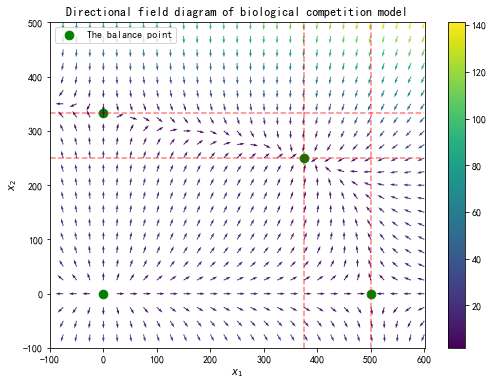
\includegraphics[width=0.6\textwidth]{img/方向场图.png}
	\caption{Directional Field Map}\label{fig:方向场图}
\end{figure}

In the fourth equilibrium point, both species exist and reach equilibrium, which belongs to the stable equilibrium point. All the arrows near this point point point to this point, which shows that even if deviate from the equilibrium point, it will eventually return to the equilibrium point.

When fungi's growth rate, moisture tolerance and other environmental conditions combined to make it move towards a stable equilibrium, the faster the ground litter decompose. When the ambient temperature and humidity change rapidly, fungi with slow growth rates and good moisture tolerance can better adapt to the environment, thus increasing the decomposition rate.
\section{Prediction to various environmental conditions}
Studies have shown that soil temperature and moisture are the key factors affecting soil microbial population composition and community structure.  It is generally believed that temperature plays a leading role in litter decomposition at large and medium scales. According to the mechanism of action, the effect of temperature on litter decomposition can be divided into two parts : direct effect and indirect effect : direct effect refers to the effect of temperature on soil and microbial related enzyme activities, when other conditions tend to be stable.  When, temperature was positively correlated with litter decomposition rate within a certain range ; Indirect effects mainly refer to the changes in litter mass, soil biology and vegetation community structure caused by long-term temperature fluctuations. These changes will lead to fundamental changes in the chemical properties and biodegradability of litter.

In the short term, elevated temperature can promote litter decomposition by increasing soil microbial activity, thereby accelerating the material cycle in forest ecosystems ; In the long time scale, the decomposition rate of litter increased exponentially with the increase of temperature. Temperature was an important limiting factor for biological activities and enzymatic reactions in the high-latitude semi-arid region, and warming was conducive to the accelerated decomposition of litter in the region.    

Precipitation and soil moisture are important environmental factors affecting the material turnover of terrestrial ecosystems, and play a controlling role in litter decomposition and related biological factors such as vegetation distribution, microbial activity and quantity. In some ecosystems of tropical and temperate regions, higher soil moisture leads to a decrease in litter decomposition rate, mainly because moisture in moist soil hinders the oxygen supply of microorganisms and inhibits the biological activity of decomposers.  

In arid and semi-arid regions, the water and heat conditions are poor, the soil organic matter is deficient, the population composition and community structure are single, and the ecological function is simple. The influence of various environmental factors on litter decomposition is complex and special, which makes the research results in this region still have great uncertainty.
\section{Effects of fungal community diversity}
In microbial groups, fungi can secrete a variety of cellulase and lignin enzymes, which can degrade the complex and stable components of cellulose, lignin and other microorganisms in forest litter layer, and promote nutrient recycling. Therefore, fungi play a crucial role in litter decomposition. Due to the specificity of biological enzymes, different types of fungi play their respective roles in different aspects of litter decomposition, and under natural conditions, microorganisms are not only a single strain to degrade litter independently, therefore, the interaction between the groups and components of each decomposer cannot be ignored. The synergistic effect between fungal communities is an important reason for the accelerated decomposition of litter. When the fungal community richness increases, the decomposition rate of litter is significantly higher than that of only the same fungal community. This is a positive competition.

The decomposition of decayed wood requires atmospheric $CO_2$ emissions to participate in the global carbon cycle. Researchers measured $CO_2$ changes in a certain period of time and compared with $CO_2$ emission indicators at the same period. It was found that samples with more fungal community richness in decayed wood emit less $CO_2$, so it can be indirectly concluded that the decomposition rate of decayed wood is negatively correlated with the fungal richness. For reasons, this is due to a ' pure diversity ' effect of biological communities, and the interference competition between fungi makes the decomposition rate of rotten wood decrease, which is a negative competition.
\begin{figure}[H]
	\centering
	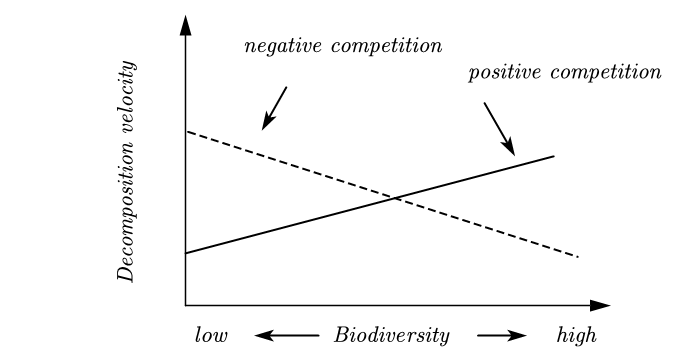
\includegraphics[width=0.6\textwidth]{img/积极消极竞争.png}
	\caption{Influence of Positive Competition and Negative Competition on Decomposition Process}\label{fig:积极消极竞争}
\end{figure}
It can be seen that positive community diversity can promote litter decomposition, and negative competitive factors inhibit litter decomposition. The schematic diagram above explains this phenomenon.
\section{Sensitivity Analysis}
From the formulas below:
$$\left\{
\begin{array}{l}
	\frac{d x}{d t}=R_{1} x\left(1-\frac{x}{\beta M_{1}}-\alpha R_{1} \frac{y}{\beta M_{2}}\right)\\
	\frac{d y}{d t}=R_{2} y\left(1-\frac{y}{\beta M_{2}}-\alpha R_{2} \frac{x}{\beta M_{1}}\right)\\
\end{array}
\right.
$$
We can find that fluctuations in $ \alpha, \beta $ may affect the simulation parameters, which may lead to inaccurate decomposition predictions. Therefore, it is necessary to test its stability. Set a random disturbance of 1\% ~ 5\% for $ \alpha, \beta $, and then import the model to predict the decomposition. The results are as follows :
\begin{table}[H]
	\centering
	\caption{The results of sensitivity evaluation}
	\begin{tabularx}{\textwidth}{@{}c *5{>{\centering\arraybackslash}X}@{}}
		\toprule[1.5pt]
		relative error & 1\%   & 2\%   & 3\%   & 4\%   & 5\% \\
		\midrule
		$\alpha$    & -0.9954\% & -1.2756\% & 1.9241\% & 3.4538\% & 3.6859\% \\
		$\beta$     & 0.4582\% & 0.9127\% & -1.5626\% & -2.8411\% & 3.1105\% \\
		\bottomrule[1.5pt]
	\end{tabularx}%
\end{table}%
We can find that the interference of the scale coefficient $\alpha, \beta$ will have a certain impact on the prediction, but the influence range is acceptable.
\section{Strengths,Weaknesses and improvement}
\subsection{Strengths}
\begin{itemize}
\item The improved Lotka-Volterra model was established by variable mapping, and the competitive relationship between two fungi with different characteristics was analyzed. 

\item The strategy of fixing one independent variable and studying the relationship between another independent variable and dependent variable overcomes the difficulty of studying multiple variables at the same time ; 

\item The influence of the difference between growth rate and moisture tolerance on the competition process was accurately simulated, and then the change of decomposition was predicted.
\end{itemize}
\subsection{Weaknesses and Improvement}
\begin{itemize}
\item When establishing the relationship between decomposition rate and other factors, less factors are considered, and the influence of external environmental factors such as temperature and humidity is not considered. 

\item The relationship between decomposition rate and growth rate, moisture tolerance is not a simple proportional relationship, but a positive correlation, our model will be directly proportional to its treatment ; 

\item If adding temperature, humidity and other environmental factors to the model, and consider the specific positive correlation, it may improve the accuracy of the model prediction.
\end{itemize}
\section{Conclusion}
Through the improved Lotka-Volterra model established by us to study the competition between the two fungi, we can draw the following conclusions : 

There were positive and negative competition relationships among fungi with different characteristics. Under the influence of positive competition relationship, litter decomposition was promoted and decomposition rate increased. Under the influence of negative competition relationship, litter decomposition was inhibited and decomposition rate decreased. When the growth rates of different fungi varied little, the total number of individuals increased steadily. When the growth rate of different fungi is quite different, the rapid growth rate is extinct, and the total number of individuals increases rapidly first, then decreases and then increases. With the increase of the difference, the litter decomposition is insufficient, and the competitive relationship is negative.

Different from the growth rate, regardless of the moisture tolerance difference of different fungi, the total number of individuals always showed a steady increase trend. The decomposition rate increased with the increase of the difference, and the decomposition was more and more sufficient. At this time, the competitive relationship was positive. 

Under the role of competition, when the growth rates of the two fungi are similar or the moisture tolerance is different, it can promote the growth of the total number of individuals and improve the decomposition efficiency. 

When ambient temperature and humidity change rapidly, fungi with slow growth rate and good moisture tolerance can better adapt to the environment, thereby increasing the decomposition rate.
\section{References}
[1] Dang C K, Schindler M, Chauvet E, et al. Temperature oscillation coupled with fungal community shifts can modulate warming effects on litter decomposition[J]. Ecology, 2009, 90(1): 122-131.

[2] See C R, Fernandez C W, Conley A M, et al. Distinct carbon fractions drive a generalisable two‐pool model of fungal necromass decomposition[J]. Functional Ecology, 2020.

[3] Martin J P, Zunino H, Peirano P, et al. Decomposition of 14C-labeled lignins, model humic acid polymers, and fungal melanins in allophanic soils[J]. Soil Biology and Biochemistry, 1982, 14(3): 289-293.

[4] Henriksen T M, Breland T A. Nitrogen availability effects on carbon mineralization, fungal and bacterial growth, and enzyme activities during decomposition of wheat straw in soil[J]. Soil Biology and Biochemistry, 1999, 31(8): 1121-1134.

[5] Tuomi M, Laiho R, Repo A, et al. Wood decomposition model for boreal forests[J]. Ecological Modelling, 2011, 222(3): 709-718.

[6] Moore J A M, Jiang J, Post W M, et al. Decomposition by ectomycorrhizal fungi alters soil carbon storage in a simulation model[J]. Ecosphere, 2015, 6(3): 1-16.

[7] Treseder K K, Lennon J T. Fungal traits that drive ecosystem dynamics on land[J]. Microbiology and Molecular Biology Reviews, 2015, 79(2): 243-262.

[8] Jacobson K, van Diepeningen A, Evans S, et al. Non-rainfall moisture activates fungal decomposition of surface litter in the Namib Sand Sea[J]. PLoS One, 2015, 10(5): e0126977.

\newpage
\section{Content in Textbook}
The carbon cycle describes the process of carbon exchange throughout the Earth ' s geochemical cycle and is an important part of life on Earth. A key group of this process Parts are the decomposition of plant materials and lignocellulose. 

Researchers examined a large number of different traits associated with each fungus and tried to determine the role of these traits in wood decomposition. 

For example, an important characteristic is mycelium elongation. Mycelium is the branch cell of fungi, which constitutes the filament and structure of fungi. Different types of hyphae play different roles in the life cycle of fungi. Mycelial elongation is essentially the growth rate of fungi.

Another feature is the density of hyphae in a given volume. These two characteristics are related to many characteristics of fungi. For example, studies have found that if the mycelium elongation is greater ( the faster growth ), fungi are more likely to decompose wood faster. Similarly, if the filaments are denser, the decomposition rate of wood is slower. In addition, these two characteristics are also related to fungal responses to different environmental conditions. 

In particular, researchers have found that fungi that better adapt to various humidity conditions tend to decompose wood slowly. Growth Fungi that are faster and more competitive than other fungi often decompose wood faster. 

Based on the above relationship, some researchers established an improved Lotka-Volterra competition model, where the litter residue and the number of fungal individuals as dependent variables, growth rate, moisture tolerance, time as independent variables, the differential equation system is as follows :
$$\left\{
\begin{array}{l}
	\frac{d x}{d t}=R_{1} x\left(1-\frac{x}{\beta M_{1}}-\alpha R_{1} \frac{y}{\beta M_{2}}\right)\\
	\frac{d y}{d t}=R_{2} y\left(1-\frac{y}{\beta M_{2}}-\alpha R_{2} \frac{x}{\beta M_{1}}\right)\\
	\frac{S}{S_m}=e^{-Q(M,R,t)}\\
	Q(M,R,t)=x+y=x(M,R,t)+y(M,R,t)\\
\end{array}
\right.
$$

In order to study the relationship between the number of litters and the growth rate and moisture tolerance of fungi under competitive conditions, the strategy of fixing one independent variable and studying the relationship between another independent variable and the dependent variable was adopted. When studying the relationship between any pair of variables, we assume that the initial number of fungi is the same.In order to facilitate the analysis, the following two kinds of simulation experiments set the second fungal growth rate and moisture tolerance higher. By changing the proportion of growth rate and moisture tolerance, the following litter residue curves were obtained ,as Fig.14
Based on the results of simulation experiments, the following conclusions are obtained : 

There were positive and negative competition relationships among fungi with different characteristics. Under the influence of positive competition relationship, litter decomposition was promoted and decomposition rate increased. Under the influence of negative competition relationship, litter decomposition was inhibited and decomposition rate decreased. When the growth rates of different fungi varied little, the total number of individuals increased steadily. When the growth rate of different fungi is quite different, the rapid growth rate is extinct, and the total number of individuals increases rapidly first, then decreases and then increases. With the increase of the difference, the litter decomposition is insufficient, and the competitive relationship is negative. 

\begin{figure}[H]
	\centering
	\subfigure[Litter Quantity Curve under 3 k Values]{
		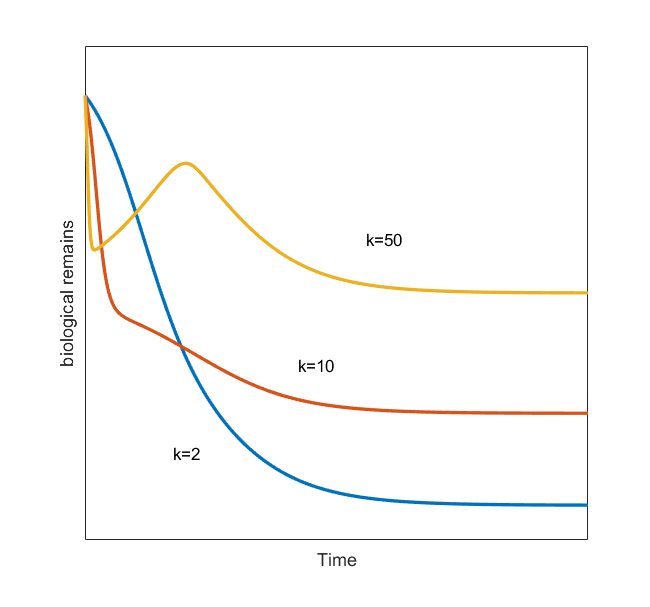
\includegraphics[width=0.45\linewidth]{img/不同k的分解曲线.png}
		%\caption{fig1}
	}
	\quad
	\subfigure[Litter Quantity Curve under 4 h Values]{
		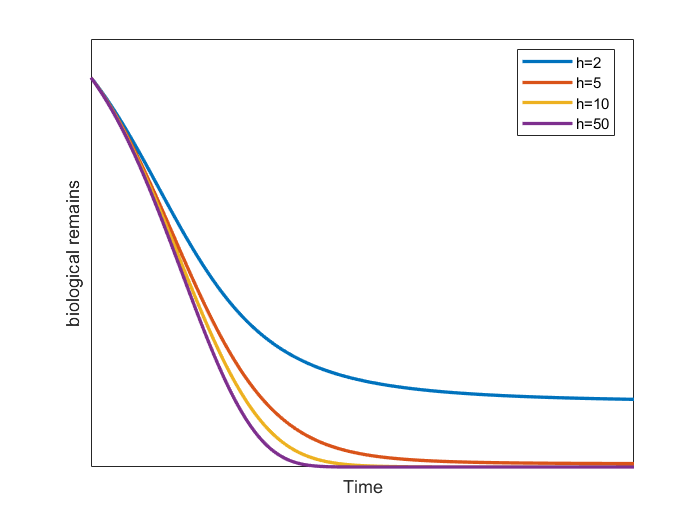
\includegraphics[width=0.45\linewidth]{img/不同h的分解曲线.png}
	}
	\caption{Decomposition in different proportions}
	
\end{figure} 



Different from the growth rate, regardless of the moisture tolerance difference of different fungi, the total number of individuals always showed a steady increase trend. The decomposition rate increased with the increase of the difference, and the decomposition was more and more sufficient. At this time, the competitive relationship was positive. 

Under the action of competition, when the growth rates of the two fungi are similar or the moisture tolerance is different, it can promote the growth of the total number of individuals and improve the decomposition efficiency.

When ambient temperature and humidity change rapidly, fungi with slow growth rate and good moisture tolerance can better adapt to the environment, thereby increasing the decomposition rate. 

In addition, studies have shown that soil temperature and moisture are key factors affecting soil microbial population composition and community structure. In the long-term scale, the decomposition rate of litter increases exponentially with the increase of temperature, and warming is conducive to the accelerated decomposition of litter in the region. In arid and semi-arid regions, higher humidity increases litter decomposition rate, but in some tropical and temperate ecosystems, higher soil moisture leads to lower litter decomposition rate, mainly due to the fact that moisture in moist soil hinders the oxygen supply of microorganisms and inhibits the biological activity of decomposers. 

Finally, the relationship between decomposition rate and biodiversity is not a simple positive correlation, when the nature of competition in biodiversity is related. When the competition among multiple organisms is positive, it can promote the decomposition rate ; When competition among multiple organisms is negative, the decomposition rate is suppressed.

%\section{Reference}
%\addcontentsline{doc}{Renference}
%\begin{thebibliography}{99}
%\bibitem[1]{1} Research and Application of Deep Learning in Image
%Recognition[D]. Wuhan: Wuhan University of Technology,
%2014. (in Chinese with English abstract)
%\bibitem[2]{2} Sun Zhijun, Xue Lei, Xu Yangming, et al. A review of
%in-depth study[J]. Computer Applied Research, 2012, 29 (8):
%2806-2810. (in Chinese with English abstract)
%\bibitem[3]{3}Ciresan, D.C., Gambardella, L.M., Giusti, A., Schmidhuber, J.: Deep neural net-
%works segment neuronal membranes in electron microscopy images. In: NIPS. pp.
%2852{2860 (2012)
%\bibitem[4]{4} Wang Chongchang, Wu Wenbo, Zhang Jianping. Remote
%sensing image classification method based on BP neural
%network[J]. Journal of Liaoning University of Engineering
%and Technology: Natural Science Edition, 2009, 28 (1): 32-
%35. (in Chinese with English abstract)
%\bibitem[5]{5}Kampffmeyer M,Salberg A B,Jenssen R.Semantic segmentation
%of small objects and modeling of uncertainty
%in urban remote sensing images using deep convolutional
%neural networks[C]//Proceedings of Computer Vision and
%Pattern Recognition Workshops,2016:680-688
%\end{thebibliography}
%[1].Li Wei. Research and Application of Deep Learning in Image
%Recognition[D]. Wuhan: Wuhan University of Technology,
%2014. (in Chinese with English abstract)
%
%[2]Sun Zhijun, Xue Lei, Xu Yangming, et al. A review of
%in-depth study[J]. Computer Applied Research, 2012, 29 (8):
%2806-2810. (in Chinese with English abstract)
%
%[3]Ciresan, D.C., Gambardella, L.M., Giusti, A., Schmidhuber, J.: Deep neural net-
%works segment neuronal membranes in electron microscopy images. In: NIPS. pp.
%2852{2860 (2012)
%	
%[4]Wang Chongchang, Wu Wenbo, Zhang Jianping. Remote
%sensing image classification method based on BP neural
%network[J]. Journal of Liaoning University of Engineering
%and Technology: Natural Science Edition, 2009, 28 (1): 32-
%35. (in Chinese with English abstract)
%	
%[5]...
%	
%[6]Kampffmeyer M,Salberg A B,Jenssen R.Semantic segmentation
%of small objects and modeling of uncertainty
%in urban remote sensing images using deep convolutional
%neural networks[C]//Proceedings of Computer V ision and
%Pattern Recognition Workshops,2016:680-688
%\section*{Appendix}

%Note : Segnet network definition and training projections are shown in the attachment code file, which lists only three main files

%\appendix
%Operating Environment:\textbf{Windows10、python3.7,anaconda2020.3}
%\section{Structure of the Project}
%\begin{figure}[H]
	%\centering
	%\includegraphics[width=0.6\textwidth]{img/xiangmu.png}
	
%\end{figure}
%\section{Definition of Unet Network}
%\lstinputlisting[language=python]{code/models/u_net.py}
%\section{Unet Network training and validation}
%\lstinputlisting[language=python]{code/train_U.py}
%\section{Unet Network Prediction}
%\lstinputlisting[language=python]{code/predict.py}


\end{document}